%%%%%%%%%%%%%%%%%%%%%%%%%%%%%%%%%%%%%%%%%%%%%%%%%%%%%%%%%%%%%%%
%
% Welcome to Overleaf --- just edit your LaTeX on the left,
% and we'll compile it for you on the right. If you open the
% 'Share' menu, you can invite other users to edit at the same
% time. See www.overleaf.com/learn for more info. Enjoy!
%
%%%%%%%%%%%%%%%%%%%%%%%%%%%%%%%%%%%%%%%%%%%%%%%%%%%%%%%%%%%%%%%
\documentclass{beamer}
\usepackage{tikz}
\usepackage{tikz-3dplot}
\usetikzlibrary{arrows.meta,calc,intersections}
\usetheme{Copenhagen}
\usecolortheme{default}
\usepackage{subcaption}
\usepackage{wrapfig}
\usepackage{svg}
\usepackage{mathtools}
\usepackage{amsmath}

\bibliographystyle{plain} % or any other style
\newcommand{\supercite}[1]{\textsuperscript{\cite{#1}}}


\setbeamerfont{footnote}{size=\tiny}

\newcommand{\lf}{\left[}
\newcommand{\rf}{\right]}
\newcommand{\ld}{\left{}
\newcommand{\rd}{\right}}
\newcommand{\lx}{\left(}
\newcommand{\rx}{\right)}

\newcommand{\red}[1]{\textcolor{red}{#1}}

% \title[Seminar Geometry: Combinatorics and Algorithms: Small-dimensional linear programming and convex hulls made easy] %optional
% {Seminar Geometry: Combinatorics and Algorithms: Small-dimensional linear programming and convex hulls made easy}

\title[Seminar Geometry: Combinatorics and Algorithms FS25] %页脚
{Small-dimensional Linear Programming and Convex Hulls Made Easy}
\subtitle{Raimund Seidel}


% \subtitle{Demonstrating the Copenhagen theme}
\author[Teng Liu] % (optional)
{Teng Liu}

% \institute[VFU] % (optional)
% {
%   \inst{1}%
%   Faculty of Physics\\
%   Very Famous University
%   \and
%   \inst{2}%
%   Faculty of Chemistry\\
%   Very Famous University
% }

\date[]{April 3rd 2025}

% Use a simple TikZ graphic to show where the logo is positioned
% \logo{\begin{tikzpicture}
% \filldraw[color=red!50, fill=red!25, very thick](0,0) circle (0.5);
% \node[draw,color=white] at (0,0) {LOGO HERE};
% \end{tikzpicture}}

%End of title page configuration block
%------------------------------------------------------------
%The next block of commands puts the table of contents at the 
%beginning of each section and highlights the current section:

\AtBeginSection[]
{
  \begin{frame}
    \frametitle{Table of Contents}
    \tableofcontents[currentsection]
  \end{frame}
}
%------------------------------------------------------------
\begin{document}
\frame{\titlepage}
%---------------------------------------------------------

\begin{frame}{Background}
	Linear programming captures one of the most canonical and influential constrained optimization problems. \\~\

	More precisely, it asks to maximize or minimize a linear objective under linear
	inequality and equality constraints.

	% \begin{figure}[ht]
	%     \centering
	%     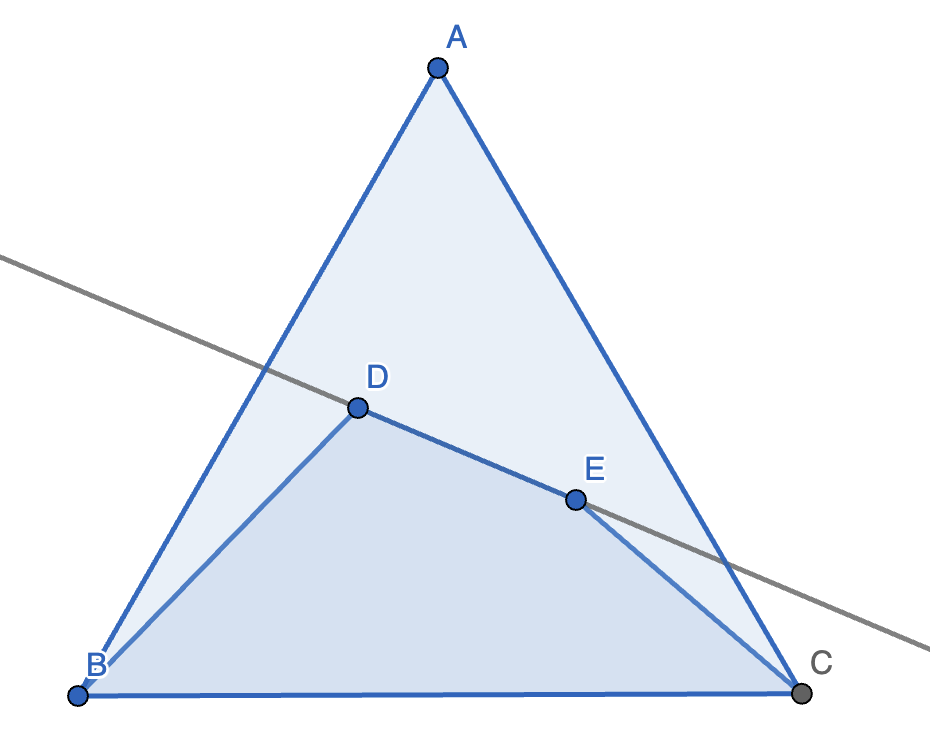
\includegraphics[width=.4\linewidth]{pre_1_1.png}
	%     \caption{Five random points on a plane}
	%     \label{fig11}
	% \end{figure}

	\begin{align*}
		\max / \min \; c^T         & x       \\
		\text{subject to} \;\;\; A & x \le e \\
		B                          & x \ge f \\
		C                          & x = g
	\end{align*}

	% this can be interpreted as maximizing profits we get from manufacturing some products with prices respectively and a certain budgets e

\end{frame}

%%% Simplex Method 1
\begin{frame}{Background - Geometrical Interpretation}
	% Every constraint corresponds to a hyperplane (a halfspace, precisely). The intersection of several halfspaces gives us a polyhedron.
	\begin{columns}
		\begin{column}{0.5\textwidth}
			\begin{align*}
				\max \; 4x+y                         \\
				\text{subject to} \;\;\; x + y \le 3 \\
				x \ge 0                              \\
				y \ge 0                              \\
			\end{align*}
		\end{column}
		\begin{column}{0.5\textwidth}
			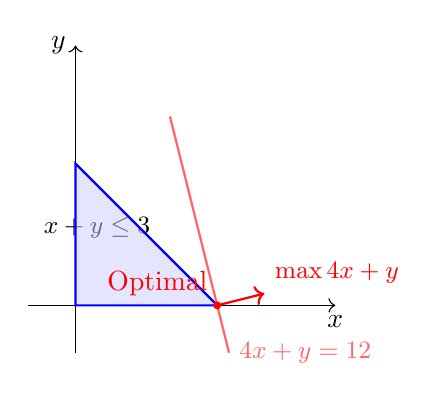
\begin{tikzpicture}[scale=0.6]

				% Axes
				\draw[->] (-1,0) -- (5.5,0) node[below] {$x$};
				\draw[->] (0,-1) -- (0,5.5) node[left] {$y$};

				% Constraints as lines
				\draw[thick, name path=c1] (0,3) -- (3,0) node[pos=0.6, above left] {\small $x + y \le 3$};

				% Feasible region (polygon)
				\fill[blue!20, opacity=0.5]
				(0,0) --
				(3, 0) coordinate (opt) --
				(0,3) --
				cycle;

				% Mark the feasible region
				\draw[thick, blue] (0,0) -- (3, 0) -- (0, 3) -- cycle;

				% Objective function direction (e.g., maximize cᵗx = 4x + y)
				\draw[->, red, thick] (3,0) -- ++(1,0.25) node[above right] {\small $\max 4x + y$};

				\draw[thick, red!60] (2,4) -- (3.25,-1) node [ right] {\small $4x+y=12$ };

				% Optimal point
				\filldraw[red] (3,0) circle (2pt) node[above left] {Optimal};

			\end{tikzpicture}
		\end{column}
	\end{columns}
\end{frame}

\begin{frame}
	\begin{center}
		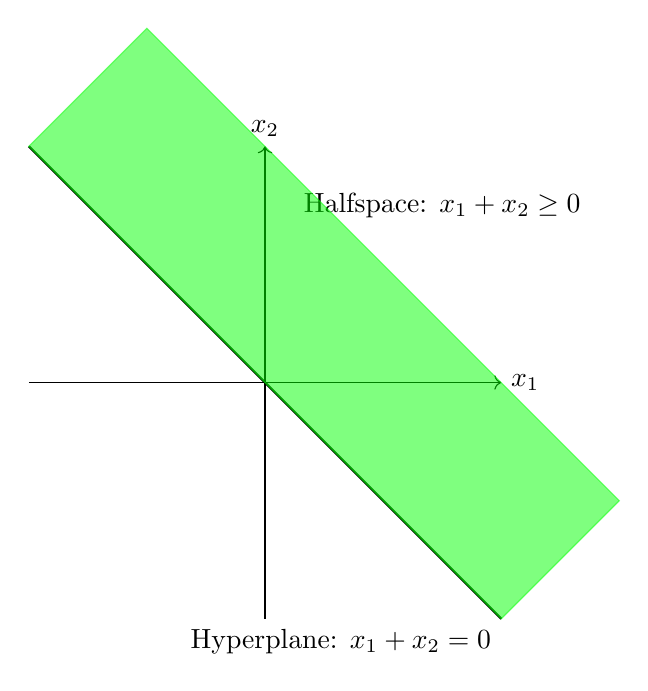
\begin{tikzpicture}[scale=1.5]
			% Axes
			\draw[->] (-2,0) -- (2,0) node[right] {$x_1$};
			\draw[->] (0,-2) -- (0,2) node[above] {$x_2$};

			% Hyperplane (line: x1 + x2 = 0)
			\draw[thick, black] (-2,2) -- (2,-2) node[below left] {Hyperplane: $x_1 + x_2 = 0$};
			\node at (1.5, 1.5) {Halfspace: $x_1 + x_2 \ge 0$};

			\filldraw[green, opacity=0.5] (-2, 2) -- (2, -2) -- (3, -1) -- (-1, 3) -- cycle;

			% \filldraw[blue, opacity=0.5] (-2, 2) -- (2, -2) -- (1, -3) -- (-3, 1) -- cycle;
			% Labels
		\end{tikzpicture}
	\end{center}
\end{frame}
\begin{frame}{Background - Facts}
	%% Simplex method is an impressive algorithm that solves lp in an intuitive way.
	%% 
	\begin{exampleblock}{Fact}
		an LP can be bounded, unbounded and infeasible.
	\end{exampleblock}
	\begin{exampleblock}{Fact}
		Optimal solution, if exists, can always be achieved by some vertex.
	\end{exampleblock}

	\begin{exampleblock}{Fact}
		If there exists any vertex with better objective value than current vertex, we always have a neighbour vertex with better value.
	\end{exampleblock}

	\pause

	Firstly select any starting vertex. \\~\

	Each step in Simplex Method move from one vertex to its neighbour with larger objective.

	% If we currently we are not in optimal vertex, there are always a neighbour vertex with better objective.
	% This can be proved intuitively with this sketch: let's assume the feasible solution (the polyhedron) is full-dimensioned.
	% Then for any vertex, if we construct a ball centering at that vertex, the intersection of ball and polyhedra
	% would be also full-dimensioned.
	% We only need to show if we take any vertex as the origin and consider the ray formed by origin and its neighbour,
	% it gives a cone, identical to the one formed by considering the intersection of all hyperplane incident to origin.

\end{frame}

%%% Simplex Method 2

\begin{frame}{Background - Simplex Method}
	Firstly select any starting vertex. \\~\

	Each step in Simplex Method move from one vertex to its neighbour with larger objective.

	\begin{figure}[r]
		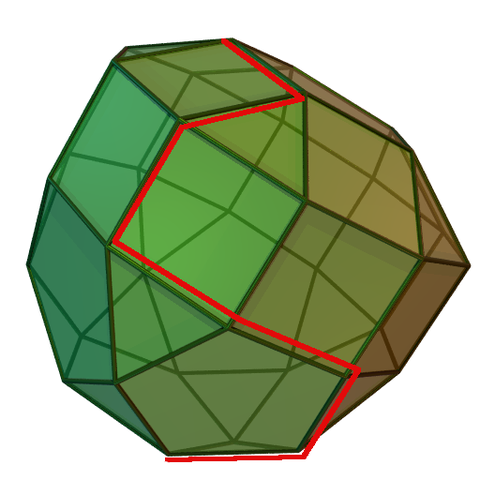
\includegraphics[width=0.4\linewidth]{pics/simplex_method.png}
		% \caption{}
		% \label{figsmallcircle}
	\end{figure}
	{\centering \tiny Fault-tolerant quantum algorithms - Scientific Figure on ResearchGate. \par}

	% If we currently we are not in optimal vertex, there are always a neighbour vertex with better objective.
	% This can be proved intuitively with this sketch: let's assume the feasible solution (the polyhedron) is full-dimensioned.
	% Then for any vertex, if we construct a ball centering at that vertex, the intersection of ball and polyhedra
	% would be also full-dimensioned.
	% We only need to show if we take any vertex as the origin and consider the ray formed by origin and its neighbour,
	% it gives a cone, identical to the one formed by considering the intersection of all hyperplane incident to origin.

\end{frame}

\begin{frame}{Background - Overview}

	\begin{table}[h]
		\centering
		\begin{tabular}{|l|l|l|l|l|}
			\hline
			\textbf{Algorithm}      & \textbf{Complexity} & \textbf{Speed} & \textbf{Approach}    \\ \hline
			\textbf{Simplex}        & Exponential         & Fast           & Edges of polyhedron  \\ \hline
			\textbf{Ellipsoid}      & Polynomial          & Slow           & Ellipsoid shrinking  \\ \hline
			\textbf{Interior Point} & Polynomial          & Fast           & Through the interior \\ \hline
		\end{tabular}
		\caption{Comparison of Famous LP Algorithms}
	\end{table}

	% Even though we have Interior Method and Ellipsoid Method, the most widely used algorithm is still Simplex Method
	% due to its efficiency in practice.
	% If we currently we are not in optimal vertex, there are always a neighbour vertex with better objective.
	% This can be proved intuitively with this sketch: let's assume the feasible solution (the polyhedron) is full-dimensioned.
	% Then for any vertex, if we construct a ball centering at that vertex, the intersection of ball and polyhedra
	% would be also full-dimensioned.
	% We only need to show if we take any vertex as the origin and consider the ray formed by origin and its neighbour,
	% it gives a cone, identical to the one formed by considering the intersection of all hyperplane incident to origin.

\end{frame}
\begin{frame}{Previous Work}
	When $d$, the dimension of LP (i.e. the number of variables), is considered to be constant,
	Megiddo showed that LP can be solved in time linear in $m$, the number of constraint.

	\vspace{\baselineskip}

	Megiddo's algorithm\supercite{M2} are complicated and the running time is doubly exponential,
	while Clarkon and Dyer improved to superexponential to $d$: e.g. $3^{d^2}$.

	\vspace{\baselineskip}

	Clarkon also proposed an algorithm\supercite{C2} with complexity $O(d^2m) + (\log m)O(d)^{d/2 + O(1)} + O(d^4 \sqrt{m} \log m)$
	but the analysis is involved.

	\vspace{\baselineskip}

	\textbf{The presented algorithm gives a simple procedure and expected complexity $O(d!m)$.}
\end{frame}

\begin{frame}{Algorithm - Sketch}

	This algorithm makes use of a very simple idea:

	\vspace{\baselineskip}

	Suppose we delete one constraint $a^T x \ge b$, and somehow managed to solve the new LP.
	Then we check if the optimum $x^*$ conforms with the deleted constraint.

	\vspace{\baselineskip}

	\begin{itemize}
		\item If it doesn't violate the constraint, i.e. $a^T x^* \ge b$, then $x^*$ is also
		      the optimum for original LP, because deleting one constraint
		      gives us a larger feasible area.
		\item If it violates the constraint, then the opt value lies on the hyperplane
		      corresponding to this constraint.  We can project the feasible area
		      onto the corresponding hyperplane, thus reducing dimension by 1. Then
		      solve the new LP problem with lower dimension.
	\end{itemize}
\end{frame}

% \begin{frame}{Algorithm - Correctness 1}
% 	Let original feasible region be $D$, feasible region after deleting constraint be $D'$, the optimum for $D'$ be $x^*$ .
% 	Clearly $D \subseteq D'$ and in this case $x^* \in D$.
% 	\begin{align*}
% 		u^T x^* \underset{\text{(i)}}{\le} \max_{D}  \underset{\text{(ii)}}{\le} \max_{D'} = u^T x^*
% 	\end{align*}
%
% 	(i): $x^* \in D$, by definition of $\max$.
%
% 	\vspace{\baselineskip}
%
% 	(ii): Optimizing on a larger area gives no worse optimal value than the original one.
% \end{frame}

\begin{frame}{Algorithm - Illustration of Second Case}
	% Let original feasible region be $D$, feasible region after deleting bounding hyperplane $h$ be $D'$, the optimum for $D'$ be $x^*$ .
	% In this case $x^* \notin D$, then $x^* \in h$.

	% \vspace{\baselineskip}
	\begin{center}
		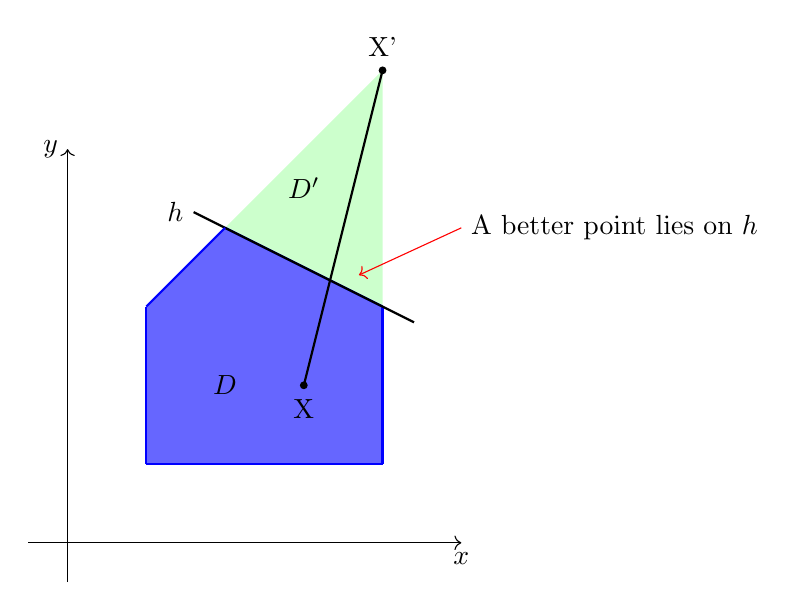
\begin{tikzpicture}
			% axes 
			\draw[->] (-0.5, 0) -- (5, 0) node[below] {$x$};
			\draw[->] (0, -0.5) -- (0, 5) node[left] {$y$};
			% Define two paths
			% \path[name path=a] (1, 0) -- (1, 7);
			% \path[name path=b] (0, 1) -- (7, 1);
			% \path[name path=c] (4, 0) -- (4, 7);
			% \path[name path=d] (5, 0) -- (0, 5);
			% \path[name path=e] (0, 1) -- (5, 6);
			%
			% \path[name intersections={of=a and e, by=A}];
			% \path[name intersections={of=b and a, by=B}];
			% \path[name intersections={of=c and b, by=C}];
			% \path[name intersections={of=d and c, by=D}];
			% \path[name intersections={of=e and d, by=E}];
			% Calculate intersection
			\coordinate (A) at (1, 1);
			\coordinate (B) at (4, 1);
			\coordinate (C) at (4, 3);
			\coordinate (D) at (2, 4);
			\coordinate (E) at (1, 3);
			\coordinate (F) at (4, 6);

			\fill[blue!60] (A) -- (B) -- (C) -- (D) -- (E) --cycle;
			\fill[green!20] (C) -- (F) -- (D) --cycle;

			% Draw the intersection point
			\draw[thick, blue] (A) -- (B);
			\draw[thick, blue] (B) -- (C);
			\draw[thick, blue] (C) -- (D);
			\draw[thick] ($ (C)!-0.2!(D) $) -- ($ (C)!1.2!(D) $) node [left] {$h$};
			\draw[thick, blue] (D) -- (E);
			\draw[thick, blue] (E) -- (A);

			\coordinate (X) at (3, 2);
			\node[circle, label=below:X, fill=black, inner sep=1pt] at (X) {};
			\coordinate (X') at (4, 6);
			\node[circle, label=above:X', fill=black, inner sep=1pt] at (X') {};

			\node at (2, 2) {$D$};
			\node at (3, 4.5) {$D'$};

			\draw[thick, black] (X) -- (X');

			\node [right] at (5, 4) {A better point lies on $h$};
			\draw[->, red] (5, 4) -- (3.7, 3.4);
		\end{tikzpicture}
	\end{center}

	% This is because if we consider the points along the line connecting
	% new LP's opt point and original LP's opt point, by convexity we have that
	% we have a better point on the hyperplane.
	% This is also not bad, at least we decrease the dimension (we restrict the problem
	% on a hyperplane, which has dimension $d - 1$), which gives us the intuition to recurssively analyse.
\end{frame}

\begin{frame}{Algorithm - Further Problems}
	Some problems left to deal with:

	\begin{itemize}
		\item What if after deletion of bounding hyperplane the new problem become unbounded?
		\item When to stop the recurssion?
		\item How can we do \textit{projection} efficiency?
		\item How to deal with infeasibility?
	\end{itemize}
\end{frame}
\begin{frame}{Algorithm - Unboundedness and Recurssion}
	The first two problems can be solved by adding a bounding box, i.e. explicit lower and upper bounds for
	variables $-\alpha \le x_i \le \alpha$ for all $d$ variables $x_i$.

	\vspace{\baselineskip}

	Recurssion stops when all original hyperplanes are deleted and it's impossible to have unbounded case.
\end{frame}
\begin{frame}{Algorithm - Projection and Infeasibility}
	Projection can be done by Gaussian elimination. Since we know a constraint has to be
	tight, we can get an equation and then we substitute it back into constraints, which
	gives us an inequality system with $d-1$ variables.

	\vspace{\baselineskip}

	Infeasibility can then be detected in dimension $1$.
\end{frame}
\begin{frame}{Algorithm - Time Complexity}
	When $d = 1$, problem can be solved in $O(m)$.

	\vspace{\baselineskip}

	When $m = 0$, problem can be solved in $O(d)$.

	\vspace{\baselineskip}

	The interesting part is when we delete a constraint and the optimum point changes.
	Since original optimum point $x$ has exactly $d$ tight constraints (i.e.
	$x$ is on exactly $d$ hyperplanes) then deleting a constraint uniformly randomly ensures
	the probability of $x'$ differs from $x$ no more than $d / m$.
\end{frame}
\begin{frame}{Algorithm - Time Complexity}
	When $d = 1$, problem can be solved in $O(m)$.

	\vspace{\baselineskip}

	When $m = 0$, problem can be solved in $O(d)$.

	\vspace{\baselineskip}

	The interesting part is when we delete a constraint and the optimum point changes.
	\red{Since original optimum point} $\red{x}$ \red{has exactly} $\red{d}$ \red{tight constraints} (i.e.
	$x$ is on exactly $d$ hyperplanes) then deleting a constraint uniformly randomly ensures
	the probability of $x'$ differs from $x$ no more than $d / m$.
\end{frame}

\begin{frame}{Algorithm - Degenerate Vertex}
	\tdplotsetmaincoords{60}{120}

	\begin{tikzpicture}[tdplot_main_coords, scale=3]

		% Base square vertices
		\coordinate (A) at (1, 1, 0);
		\coordinate (B) at (-1, 1, 0);
		\coordinate (C) at (-1, -1, 0);
		\coordinate (D) at (1, -1, 0);

		% Tip of the cone
		\coordinate (O) at (0, 0, 1.5);

		% Draw base
		% \draw[thick] (A) -- (B) -- (C) -- (D) -- cycle;

		% Draw sides
		\draw[fill=gray!30, opacity=0.8] (O) -- (B) -- (C) -- cycle;
		\draw[fill=gray!30, opacity=0.8] (O) -- (C) -- (D) -- cycle;
		\draw[fill=gray!30, opacity=0.8] (O) -- (D) -- (A) -- cycle;
		\draw[fill=gray!30, opacity=0.8] (O) -- (A) -- (B) -- cycle;

		\filldraw[fill=red] (O) circle (2pt);

	\end{tikzpicture}

\end{frame}

\begin{frame}{Algorithm - Time Complexity}
	Even if there are $k > d$ constraints are tight at $x$, the optimum point for original LP, at most $d$ of them
	has the property that deleting it leads a better optimum.

	\vspace{\baselineskip}

	% \begin{align*}
	% 	\exists v, \;\; & a_1^Tv > 0   \\
	% 	                & a_2^Tv \le 0 \\
	% 	                & \cdots       \\
	% 	                & a_k^Tv \le 0
	% \end{align*}
\end{frame}
\begin{frame}{Algorithm - Time Complexity}
	\[
		T(d, m) \le
		\begin{cases}
			O(m)                         & \text{if } d = 1, \\
			O(d)                         & \text{if } m = 1, \\
			T(d, m - 1) + O(d) + \dfrac{d}{m} O(dm) +        \\
			\dfrac{d}{m} T(d - 1, m - 1) & \text{otherwise}.
		\end{cases}
	\]

	Expand everything and we get:

	\begin{align*}
		T(d, m) = O(\sum_{1\le i \le d} \frac{i^2}{i!} d! m) = O(d! m)
	\end{align*}

\end{frame}

\begin{frame}{Convex Hull}
	For a point set $S$ on $\mathbb{R}^d$, assuming general position ( no $d + 1$ points lie in a common hyperplane), we consider
	construction of convex hull $P$ of point set $S$.

	\vspace{\baselineskip}


	\begin{figure}[h]
		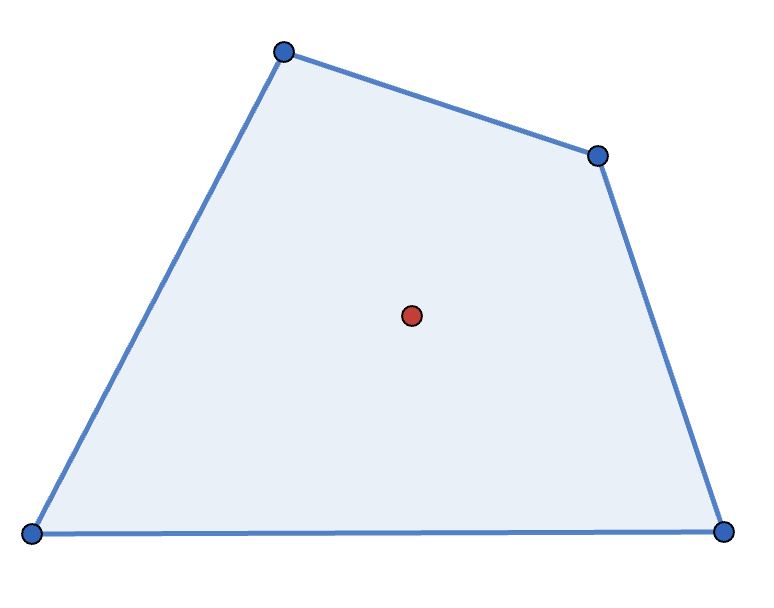
\includegraphics[width=0.4\linewidth]{pics/not_4hole.png}
		% \caption{Convex hull structure: 5, 4, 3, 2.  There are 73 different structures for $n=17$.}
		% \label{figstruct}
	\end{figure}
\end{frame}

\begin{frame}{Terminology}
	Let $p$ be some point in $\mathbb{R}^d$ in general position with respect to $S$.

	\vspace{\baselineskip}

	We call a facet $F$ of $P$ \textit{visible} from $p$ iff the hyperplane spanned by $F$
	seperates $P$ and $p$; a facet \textit{obscured} otherwise.

	\vspace{\baselineskip}

	We call a face $G$ \textit{visible} from $p$ iff it's only containted in facets of $P$ that are visible from $p$.
	\textit{Obscured} faces are defined analogously.
	We call $G$ a face \textit{horizon} iff it's contained in some visible and some obscured facet.
\end{frame}

\tikzstyle{vertex}=[
circle,
draw=black,
fill=black,
inner sep=0pt,    % No extra padding
minimum size=1pt, % Diameter = 6pt (radius = 3pt)
text=white,
font=\footnotesize
]

\begin{frame}
	\begin{center}
		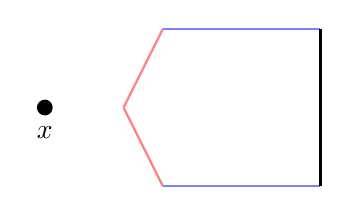
\begin{tikzpicture}[scale=1]

			\coordinate (a) at (0, 0);
			\coordinate (b) at (0, 2);
			\coordinate (c) at (2, 0);
			\coordinate (d) at (2, 2);
			\coordinate (e) at (-0.5, 1);
			\draw[thick,red!50] (a) -- (e);
			\draw[thick,red!50] (b) -- (e);
			\draw[thick,blue!50] (b) -- (d);
			\draw[thick,blue!50] (a) -- (c);
			\draw[thick,black] (c) -- (d);
			% \draw[fill=blue!50] (b) -- (c);

			% \node[fill=black,circle,inner sep=0,minimum size=0.01] at (-2, 1) {$x$};
			\fill[black] (-1.5, 1) circle[radius=0.1] node[label=below:$x$] {};

		\end{tikzpicture}
	\end{center}
	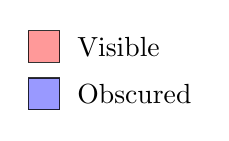
\begin{tikzpicture}[scale=1]
		\draw[fill=red!50, opacity=0.8] (0,0.3) rectangle +(0.4,0.4);
		\node[anchor=west] at (0.5,0.5) {Visible};

		\draw[fill=blue!50, opacity=0.8] (0,-0.3) rectangle +(0.4,0.4);
		\node[anchor=west] at (0.5,-0.1) {Obscured};

	\end{tikzpicture}

\end{frame}

\begin{frame}
	\begin{center}
		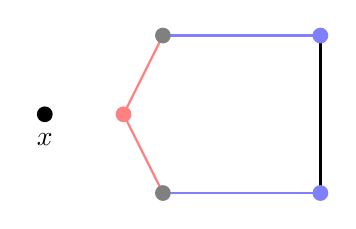
\begin{tikzpicture}[scale=1]

			\coordinate (a) at (0, 0);
			\coordinate (b) at (0, 2);
			\coordinate (c) at (2, 0);
			\coordinate (d) at (2, 2);
			\coordinate (e) at (-0.5, 1);
			\draw[thick,red!50] (a) -- (e);
			\draw[thick,red!50] (b) -- (e);
			\draw[thick,blue!50] (b) -- (d);
			\draw[thick,blue!50] (a) -- (c);
			\draw[thick,black] (c) -- (d);
			% \draw[fill=blue!50] (b) -- (c);

			% \node[fill=black,circle,inner sep=0,minimum size=0.01] at (-2, 1) {$x$};
			\fill[black] (-1.5, 1) circle[radius=0.1] node[label=below:$x$] {};

			\fill[red!50] (e) circle[radius=0.1] node[] {};
			\fill[gray] (a) circle[radius=0.1];
			\fill[gray] (b) circle[radius=0.1];
			\fill[blue!50] (c) circle[radius=0.1];
			\fill[blue!50] (d) circle[radius=0.1];

		\end{tikzpicture}
	\end{center}
	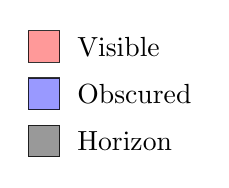
\begin{tikzpicture}[scale=1]
		\draw[fill=red!50, opacity=0.8] (0,0.3) rectangle +(0.4,0.4);
		\node[anchor=west] at (0.5,0.5) {Visible};

		\draw[fill=blue!50, opacity=0.8] (0,-0.3) rectangle +(0.4,0.4);
		\node[anchor=west] at (0.5,-0.1) {Obscured};

		\draw[fill=gray, opacity=0.8] (0,-0.9) rectangle +(0.4,0.4);
		\node[anchor=west] at (0.5,-0.7) {Horizon};

	\end{tikzpicture}

\end{frame}
\begin{frame}{Convex Hull - Facts}
	Consider an incremental algorithm, from original convex hull $P$ to construct $P' = conv(P \bigcup x)$ where $x$
	is the new point, and we have the following observations:
	\begin{itemize}
		\item no visible face of $P$ is a face of $P'$;
		\item all obsecured and horizon faces of $P$ are faces of $P'$;
		\item for each horizon face $G$ of $P$, the pyramid $conv(G \bigcup x)$ is a face of $P'$;
		\item this yields all faces of $P'$.
	\end{itemize}
\end{frame}

\begin{frame}
	\begin{center}
		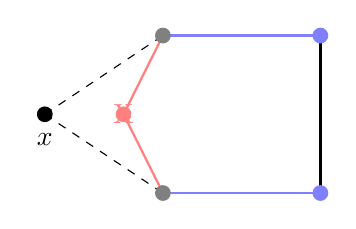
\begin{tikzpicture}[scale=1]

			\coordinate (a) at (0, 0);
			\coordinate (b) at (0, 2);
			\coordinate (c) at (2, 0);
			\coordinate (d) at (2, 2);
			\coordinate (e) at (-0.5, 1);
            \coordinate (new) at (-1.5, 1);
			\draw[thick,red!50] (a) -- (e);
			\draw[thick,red!50] (b) -- (e);
			\draw[thick,blue!50] (b) -- (d);
			\draw[thick,blue!50] (a) -- (c);
			\draw[thick,black] (c) -- (d);
			% \draw[fill=blue!50] (b) -- (c);

			% \node[fill=black,circle,inner sep=0,minimum size=0.01] at (-2, 1) {$x$};
			\fill[black] (-1.5, 1) circle[radius=0.1] node[label=below:$x$] {};

            \draw[dashed] (new) -- (a);
            \draw[dashed] (new) -- (b);

			\fill[red!50] (e) circle[radius=0.1] node[] {X};
			\fill[gray] (a) circle[radius=0.1];
			\fill[gray] (b) circle[radius=0.1];
			\fill[blue!50] (c) circle[radius=0.1];
			\fill[blue!50] (d) circle[radius=0.1];

		\end{tikzpicture}
	\end{center}
	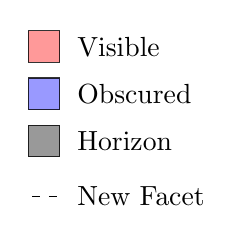
\begin{tikzpicture}[scale=1]
		\draw[fill=red!50, opacity=0.8] (0,0.3) rectangle +(0.4,0.4);
		\node[anchor=west] at (0.5,0.5) {Visible};

		\draw[fill=blue!50, opacity=0.8] (0,-0.3) rectangle +(0.4,0.4);
		\node[anchor=west] at (0.5,-0.1) {Obscured};

		\draw[fill=gray, opacity=0.8] (0,-0.9) rectangle +(0.4,0.4);
		\node[anchor=west] at (0.5,-0.7) {Horizon};

        \draw[dashed] (0.05, -1.4) -- (0.4, -1.4);
		\node[anchor=west] at (0.5,-1.4) {New Facet};

	\end{tikzpicture}

\end{frame}
\begin{frame}{Convex Hull Sketch}
	\begin{enumerate}
		\item Locate a facet $F$ of $P$ visible from $x$. If no such $F$ exists then $P' = P$.
		\item Determine set of facets and ridges of $P$ visible from $x$ and horizon ridges.
		      Delete all visible facets and ridges.
		\item For each horizon ridge $G$, generate new facet $conv(G \bigcup \{ x \})$ (a new node for facet graph).
		\item Generate new edges (i.e. ridges of $P'$) for new node in facet graph.
	\end{enumerate}
\end{frame}
\begin{frame}{Convex Hull - Step 1}
	Step $1$: Locate a facet $F$ of $P$ visible from $x$. If no such $F$ exists then $P' = P$.

	\vspace{\baselineskip}

	This can be done by linear programming with $d + 1$ variables indicating parameters of hyperplane and
	each vertex gives a seperating constraint (the target hyperplane should seperate all vertices and $x$).
	The objective function is the max distance of vertices and target hyperplane.

	\vspace{\baselineskip}

	If such hyperplane exists, it must touch some visible vertex $v$.
	Then we iterate all facets containing $v$, among which we can find a seperating facet.

	\vspace{\baselineskip}

	According to the LP algorithm, \textbf{this can be done in $O(i)$ time in $i$-th iteration}.
\end{frame}
\begin{frame}{Convex Hull - Step 2}
	Step $2$: Find all visible facets and ridges, then delete them.

	\vspace{\baselineskip}

	This can be done by Depth-First-Search from the facet determined in step $1$.
	\textbf{The time cost is proportional to number of visible facets}, which can be accounted
	into the creation step of these facets, amortizedly speaking.
\end{frame}
\begin{frame}{Convex Hull - Time Complexity}
	Step $3$: Generate new facet for each horizon ridge.

	\vspace{\baselineskip}

	All horizon ridges can found in step $2$ and adding new nodes in facet graph
	\textbf{cost clearly time proportional to number of new facets} $N_i$.
\end{frame}
\begin{frame}{Convex Hull - Time Complexity}
	Step $4$: Generate new edges in facet graph.

	\vspace{\baselineskip}

	Here we need to pair up facets (i.e. nodes in facet graph) to add new edges.
	For each new facet, we can iterate all ridges (represented as $d-1$-tuple of vertices index).
	Then by Radix Sort or Trie Tree we can simply identify the corresponding old facet of each ridge.

	\vspace{\baselineskip}

	\textbf{This can be done in $O(i + N_i)$ time.}
\end{frame}
\begin{frame}{Convex Hull - Time Complexity}
	Put points of $S$ in random order $p_1, \cdots, p_n$.

	\vspace{\baselineskip}

	For $i$-th iteration, we compute $P_i$ out of $P_{i-1}$ and the running time is $O(i + N_i)$, where $N_i$ is the number of
	of facets constaining $p_i$ in $P_i$.

	\vspace{\baselineskip}

	There are at most $i^{\lfloor \frac{d}{2} \rfloor}$ facets and the probability that a vertex is contained in a facet
	is $d / i$. So the expected running time for this iteration is $i^{\lfloor \frac{d}{2} \rfloor - 1}$, leading to total complexity of $n^{\lfloor \frac{d}{2} \rfloor }$.

    Notice this procedure doesn't work when $d \le 3$.
\end{frame}
\begin{frame}{Smallest Enclosing Circle}
    An algorithm inspired by this paper is proposed by Emo Welzl\cite{emo}.

	\begin{block}{Smallest Enclosing Circle}
		Given a set of points $P$ in Euclidean plane, compute the smallest circle that contains them all.
	\end{block}

	\begin{figure}[r]
		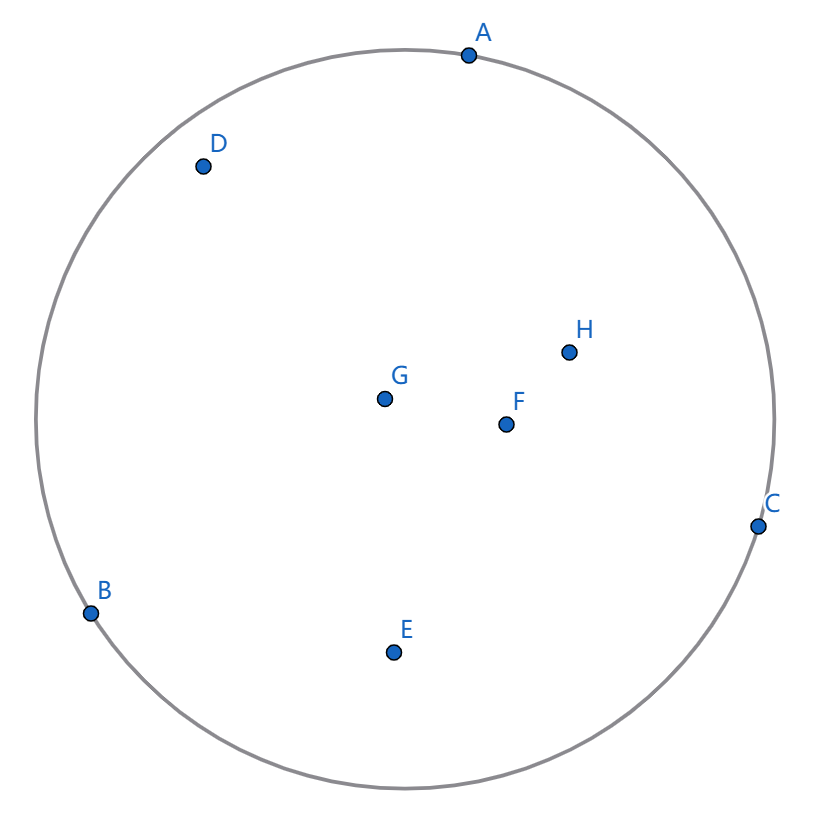
\includegraphics[width=0.3\linewidth]{pics/smallest_enclosing_circle_illustration.png}
		% \caption{}
		% \label{figsmallcircle}
	\end{figure}

	% Given first $i$ points, $\text{Pr}\lf \text{No.}(i+1) \text{ point falls in the interior of circle } C_{i+1} \rf = \;?$ \\~\

	% Given first $i+1$ points, $\text{Pr}\lf \text{No.}(i+1) \text{ point falls in the interior of circle } C_{i+1} \rf = \;?$

	% in fact, the two algorithms shares a trick in analysing some algos in common, it's called backward analysis by Seidel. the details are in depth explained in another paper where the author listed several other algorithms that backward analysis can also apply, either to give a simple proof for a previously complicated algorithm or a completely new, yet still simple proof for a new algorithm.

	% the first one is difficult to calculate because it's intrinsicly difficult. The probability differs when we have different set of first i points. So it's indeed hard to give a probability for any set of first i points, but we don't care about the probability for any specific set of first i points whatsoever: we care about only the expectation: as long as the expectation of this probability among all possible sets of first i points is bounded by some value then we are happy.

	% the second one is smarter in the sense that it doesn't depend on the set of i+1 points. whichever we choose we always have the same probability

	% here we need two pictures illustrating this:

\end{frame}

\begin{frame}{Smallest Enclosing Circle}

	An efficient random algorithm with surprisingly simple procedure:

	\begin{figure}[h]
		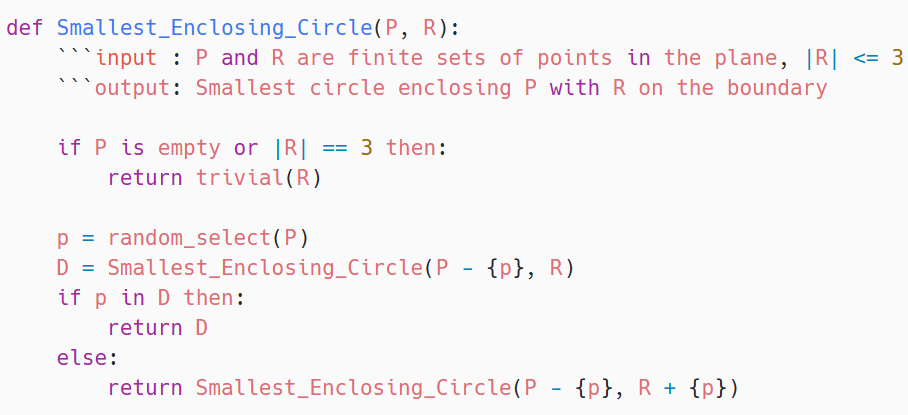
\includegraphics[width=1.0\linewidth]{pics/smallest_enclosing_circle_psudocode.png}
		% \caption{Convex hull structure: 5, 4, 3, 2.  There are 73 different structures for $n=17$.}
		% \label{figstruct}
	\end{figure}

	% Given first $i$ points, $\text{Pr}\lf \text{No.}(i+1) \text{ point falls in the interior of circle } C_{i+1} \rf = \;?$ \\~\

	% Given first $i+1$ points, $\text{Pr}\lf \text{No.}(i+1) \text{ point falls in the interior of circle } C_{i+1} \rf = \;?$

	% in fact, the two algorithms shares a trick in analysing some algos in common, it's called backward analysis by Seidel. the details are in depth explained in another paper where the author listed several other algorithms that backward analysis can also apply, either to give a simple proof for a previously complicated algorithm or a completely new, yet still simple proof for a new algorithm.

	% the first one is difficult to calculate because it's intrinsicly difficult. The probability differs when we have different set of first i points. So it's indeed hard to give a probability for any set of first i points, but we don't care about the probability for any specific set of first i points whatsoever: we care about only the expectation: as long as the expectation of this probability among all possible sets of first i points is bounded by some value then we are happy.

	% the second one is smarter in the sense that it doesn't depend on the set of i+1 points. whichever we choose we always have the same probability

	% here we need two pictures illustrating this:

\end{frame}

\begin{frame}[allowframebreaks]{References}
	\bibliography{ref}
\end{frame}
\end{document}
